\chapter{Nasadenie do vyučovania}
\label{chap:nasadenie_do_vyucovania}

Aby bola preverená celková kvalita a využiteľnosť virtuálneho laboratória, bol nástroj EVE-ng nasadený na vypracovávanie rôznych topológii z vybraných predmetov, ktoré sú opísané v nasledujúcich častiach tejto kapitoly. Zároveň budú popísané aj problémy proces nasadzovania sprevádzali. Predmety sú uvedené v poradí podľa toho, v akom čase bol nástroj EVE-ng na nich používaný. Návod na vytvorenie vlastnej topológie je uvedený v kapitole \ref{chap:pouzivanie_eve_ng}.





\section{Projektovanie sietí 2}

V rámci predmetu Projektovanie sietí 2 bol nástroj EVE-ng nasadený do vyučovania na vypracovávanie topológii s pokročilejšími sieťovými technológiami. Topológie boli spustené na virtuálnom EVE-ng serveri.

V EVE-ng boli úspešne dokončené semestrálne práce s témou \emph{VPLS} a \emph{Seamless MPLS}. Téma \emph{EVPN} bola vypracovávaná v nástroji \emph{ViRo2}.

Topológie semestrálnych prác sa skladali z týchto zariadení:

\begin{itemize}[noitemsep]
    \item Cisco IOL smerovač - VPLS, Seamless MPLS
    \item Cisco CSR - VPLS
    \item Juniper Olive - Seamless MPLS
    \item Juniper vMX 15 - VPLS
    \item Nokia VSR - EVPN
\end{itemize}

Vypracovávanie semestrálnych prác sa však nezaobišlo bez komplkácii. Neustále bola zapracovávaná spätná väzba ostatných skupín ohľadom používania nástroja EVE-ng a podporovaných technológii zariadení. Zistilo sa, že virtuálna inštalácia EVE-ng neposkytuje dostatočný výkon, ktorý bol potrebný na vypracovanie všetkých semestrálnych prác. Preto bol vytvorený fyzický EVE-ng server, ktorý bol nasadený na nasledujúcom predmete, Počítačové siete 2.





\section{Počítačové siete 2}

V rámci predmetu Počítačové siete 2 bol nástroj EVE-ng nasadený do vyučovania na vypracovávanie topológii s \emph{point-to-point} technológiami. Topológie boli spustené na fyzickom EVE-ng serveri. V prípade zlyhania EVE-ng boli pripravené aj záložné topológie v nástroji Dynamips/Dynagen.

Najprv bola vytvorená základná topológia, znázornená na obrázku \ref{obr:eve_ng_ppp_zakladna_topo_v2}. Tá pozostávala zo štyroch Cisco IOL smerovačov a dvoch koncových zariadení s operačným systémom Alpine Linux. Cisco IOL smerovač bol vybraný, pretože ako jediný podporoval sériové rozhrania a \emph{point-to-point} technológie. Koncové zariadenie Alpine Linux bolo vybrané pre svoju nenáročnosť na systémové zdroje.

Celkovo bolo vytvorených 8 zhodných topológii, ktoré medzi sebou zdieľali jeden učiteľský smerovač. V topológii sa celkovo nachádzalo 33 Cisco IOL smerovačov a 16 koncových staníc. Celková topológia sa nachádza na obrázku \ref{obr:eve_ng_ppp_celkova_topo_v2}.

\begin{figure}
    \centering
    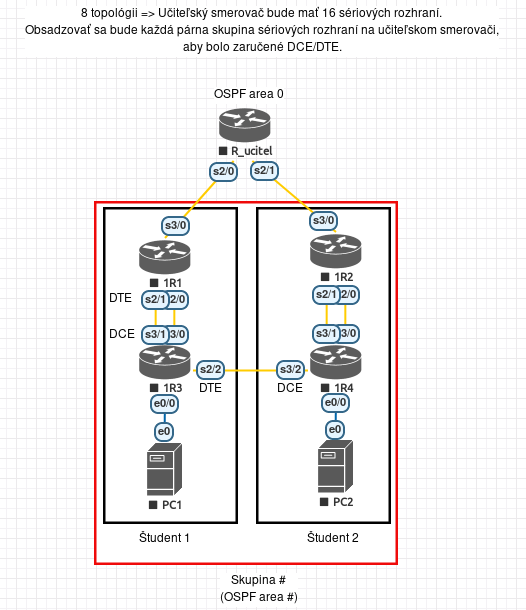
\includegraphics[width=0.6\textwidth,trim={2cm 0cm 2cm 2.5cm},clip]{eve_ng_ppp_zakladna_topo_v2}
    \caption{Základná PPP topológia}
    \label{obr:eve_ng_ppp_zakladna_topo_v2}

    \vspace{3cm}

    \centering
    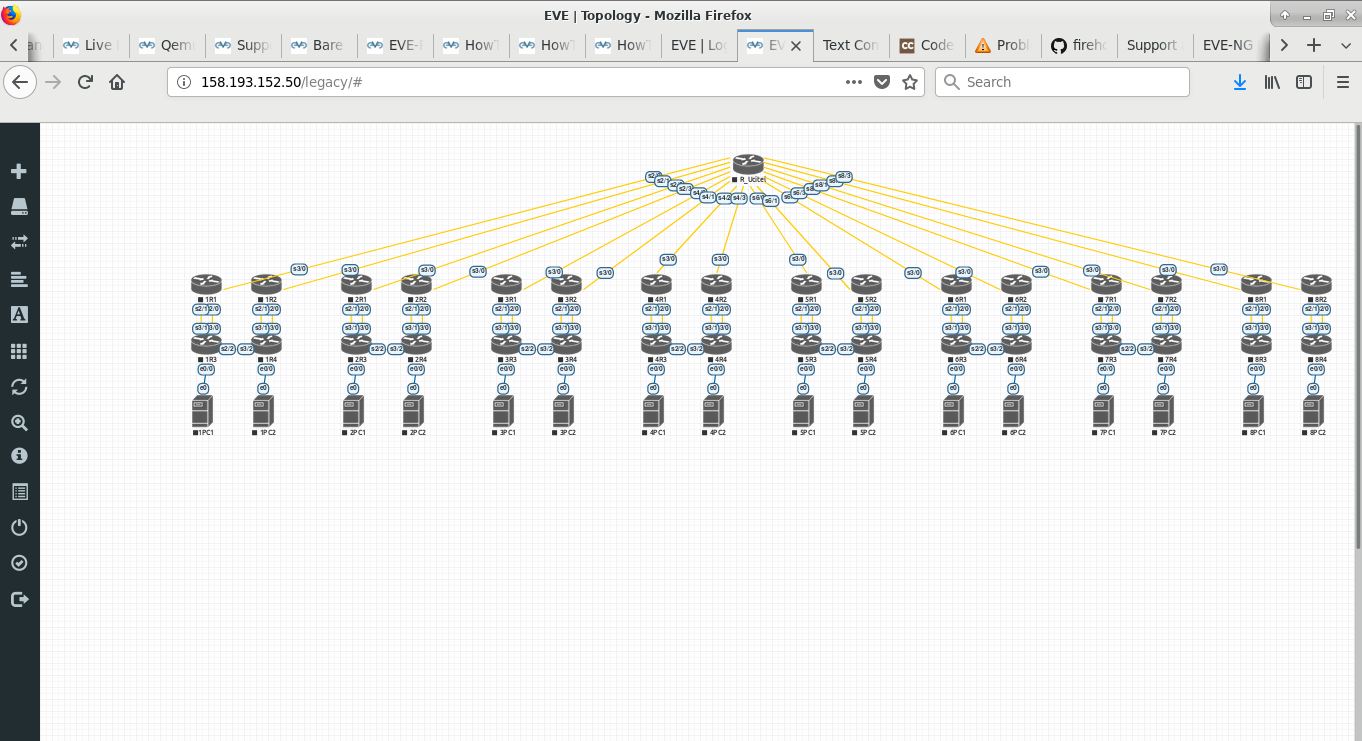
\includegraphics[width=1.0\textwidth,trim={4cm 10cm 0.5cm 4cm},clip]{eve_ng_ppp_celkova_topo_v2}
    \caption{Celková PPP topológia}
    \label{obr:eve_ng_ppp_celkova_topo_v2}
\end{figure}

IOL smerovače fungovali, až na príkaz \texttt{clock rate} na sériových rozhraniach, bez chyby. Ukázalo sa, že nastavenie DCE/DTE závisí od párnosti čísla skupiny. Párne číslo skupiny sériových rozhraní bude vždy DTE, nepárne vždy DCE, ako je zrejmé z obrázku \ref{obr:eve_ng_dce_dte_2E8S}. Rozdelenie sériových rozhraní na DCE/DTE nezávislé od počtu ethernetových alebo sériových skupín, čo potvrdzuje obrázok \ref{obr:eve_ng_dce_dte_1E8S}. Nastavenie DTE/DCE módu pre sériové rozhrania je v EVE-ng pri Cisco IOL smerovačoch pevne dané a nedá sa zmeniť, na čo treba myslieť pri návrhu topológie. Pre porovnanie, v nástroji Dynamips/Dynagen sa dá DCE/DTE mód na jednotlivých sériových rozhraniach ľubovoľne meniť.

\begin{figure}
    \centering
    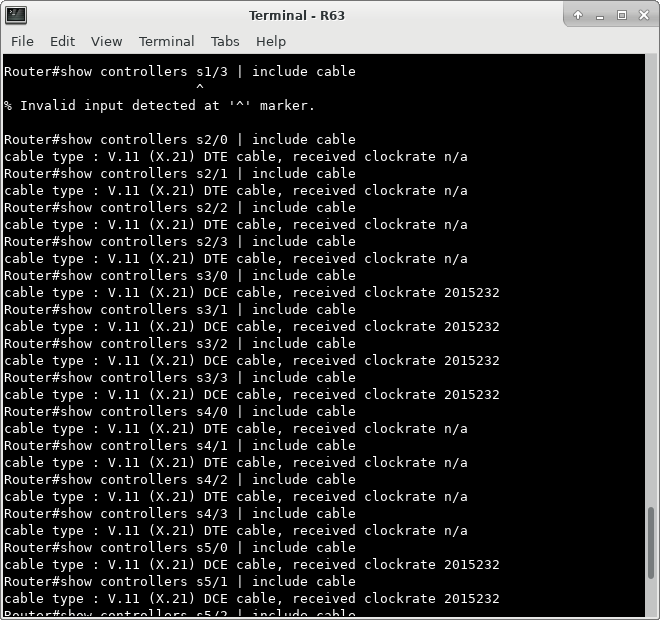
\includegraphics[width=0.7\textwidth]{eve_ng_dce_dte_2E8S}
    \caption{Typy sériových rozhraní na IOL smerovači - 2 ethernetové + 8 sériových skupín}
    \label{obr:eve_ng_dce_dte_2E8S}

    \vspace{1cm}

    \centering
    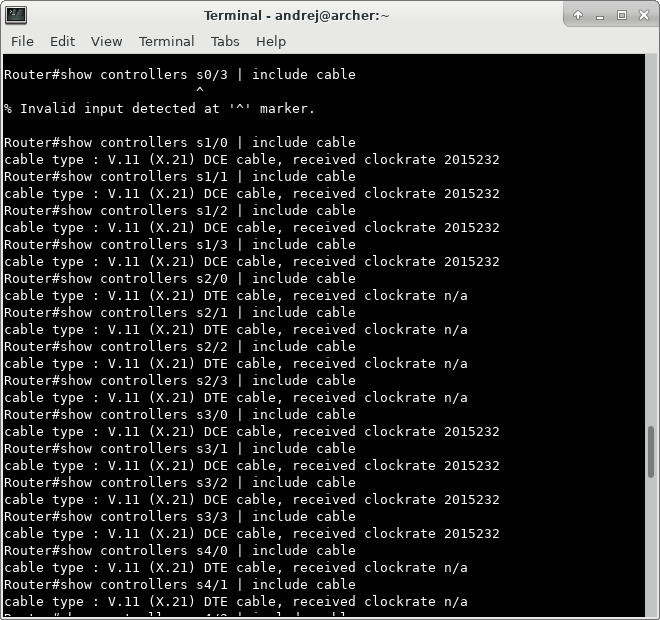
\includegraphics[width=0.7\textwidth]{eve_ng_dce_dte_1E8S}
    \caption{Typy sériových rozhraní na IOL smerovači - 1 ethernetová + 8 sériových skupín}
    \label{obr:eve_ng_dce_dte_1E8S}
\end{figure}

V jednej študentskej skupine sa vyskytol problém s jednosmernou PAP autentifikáciou študentského smerovača voči učiteľskému (R\_Ucitel(s4/1)-5R2(s2/1)). Príkaz \\\texttt{debug ppp authentication} hlásil chybu pri autentifikácii. Riešenie spočívalo v odstránení používateľa, vypnutí \emph{ppp} konfigurácie a vypnutí rozhraní. Všetky tieto kroky boli vykonané aj na učiteľskom, aj na študentskom smerovači. Následne sa konektivita obnovila a spojenie pomocou PAP autentifikácie sa úspešne nadviazalo.

Je možné, že problémy vznikli aj kvôli tomu, že medzi študentským a učiteľským smerovačom boli na oboch stranách sériové rozhrania párnej skupiny t.j. obidva konce linky boli typu DTE. Niektoré skupiny študentov boli tiež pripojené k učiteľskému smerovaču sériovým rozhraním z párnej skupiny, ale takéto problémy nezaznamenali. Podobne tomu bolo aj pri prepojení Cisco IOL smerovačov rozhraniami DCE.

Z toho vyplýva, že Cisco IOL smerovače v EVE-ng majú pri prepojení dvoch smerovačov sériovou linkou s rovnakým módom nedefinované správanie. Tomu sa dá predísť vhodným návrhom topológie. Ten spočíva v tom, že sériové rozhrania medzi smerovačmi kombinujeme tak, aby bolo prepojené vždy sériové rozhranie párnej skupiny na jednom smerovači so sériovým rozhraním nepárnej skupiny na inom smerovači t.j. \emph{Serial2/x} (DCE) na prvom smerovači sa musí pripojiť napr. k \emph{Serial3/x} na druhom. V takom prípade DCE koniec po nastavení \texttt{clock rate} v príkaze \texttt{show controllers} zobrazí nastavený atribút \emph{received clockrate}, DTE koniec naproti tomu zobrazí hodnotu \emph{n/a}. Napriek tomu konektivita po správnom nastavení IP adries a zapnutí rozhraní bola aktívna.

Komplikácie s DCE/DTE a PPP autentifikáciou boli prítomné v prvom návrhu topológie, ktorý je znázornený na obrázku \ref{obr:eve_ng_ppp_zakladna_topo_v1}.

Pri testovaní DCE/DTE rozhraní sme narazili na obmedzenie nástroja EVE-ng. Community verzia je totiž dovoľuje v jednej topológii mať spustených najviac 63 zariadení. Po spustení 64. sa na niekoľko sekúnd spustí, ale nakoniec sa automaticky vypne. Community verzia vie spustiť aj viac ako 64 zariadení v jednej topológii, ale vo výsledku sa spustia len niektoré, na prvý pohľad náhodne vybrané zariadenia. Avšak tie zariadenia, ktoré sa spustia, pracujú štandardným spôsobom. Uvedený problém sa nám nepodarilo vyriešiť ani rozšírením rozsahu portových čísel pre zariadenia v topológii.
  
Zmerané boli aj systémové požiadavky celkovej topológie na fyzickom EVE-ng serveri. Po vyhodnotení výsledkov merania sme zistili, že celá topológia, 33 Cisco IOL smerovačov a 16 koncových zariadení Alpine Linux, sa spúšťala približne 2 minúty, spotrebovala 13GB operačnej pamäte a procesor vyťažovala na 21\%. Celkovo by sme podľa celkového vyťaženia CPU mohli spustiť 4 takéto topológie, avšak množstvo operačnej pamäte by dovoľovalo spustiť iba 3. Tabuľkový dokument s výsledkami merania systémových požiadaviek topológie je prítomný v kapitole \ref{chap:cd} v bode \ref{item:nasadenie_ps2_benchmark}

Spomenutý súbor ukazuje veľké rozdiely v meraniach využitia operačnej pamäte medzi nástrojmi \emph{ps} a \emph{ps\_mem} v hárku \emph{VstupVystup}, hoci sa merala rovnaká množina procesov. Po manuálnom overení sa ukázalo, že prvý menovaný nástroj vykazoval presnejšie výsledky, preto boli pri odhadoch použité ním namerané hodnoty.

\begin{figure}
    \centering
    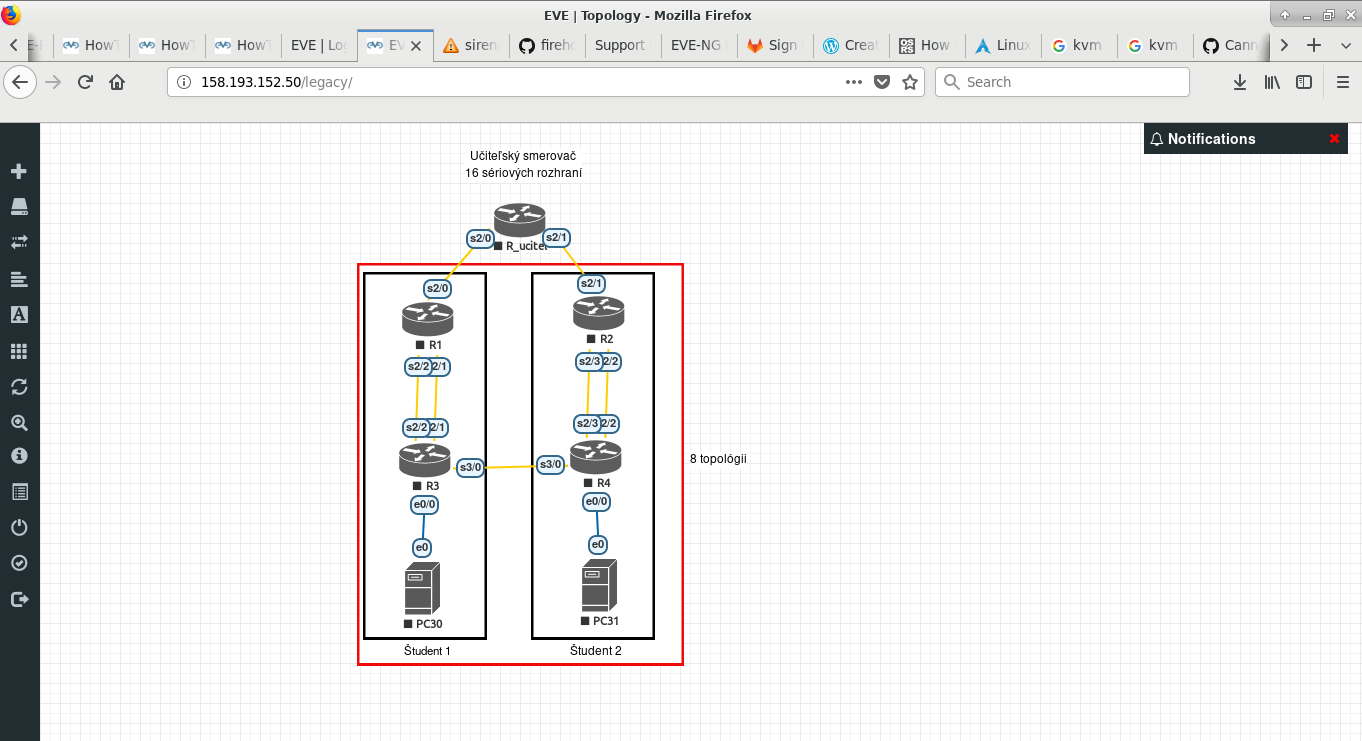
\includegraphics[width=0.5\textwidth,trim={12cm 2cm 23.7cm 7cm},clip]{eve_ng_ppp_zakladna_topo_v1}
    \caption{Základná PPP topológia - prvotný návrh}
    \label{obr:eve_ng_ppp_zakladna_topo_v1}
\end{figure}





\section{Projektovanie sietí 1}

{\huge TODO -dorobiť budúci týždeň - konzultovať s Marekom}

-nasadiť na jedno cvičenie Projektovania sietí 1
-1 používateľ môže mať otvorenú iba 1 topológiu, ktorá je obmedzená na 63 súčasne spustených zariadení. Ak treba mať spustených 100 smerovačov, 10 smerovačov v 10 topológiách, potom je potrebné vytvoriť 2 používateľské účty - polovicu topológii spustiť v jednom a polovicu v druhom používateľskom účte.


Použité zariadenia:
-Cisco IOL prepínač - 2x10
-Cisco IOL smerovač - 2x10
-Cisco 3725 - 2x10
-Cisco 7206 VXR - 2x10
-Cisco vIOS smerovač 1x10
-Cisco vIOS prepínač 2x10

Medzi R2, R3 a R4 bude bridge sieť namiesto prepínača, aby sme šetrili systémové prostriedky

Cisco IOL zariadenia mali 3 Ethernet skupiny, aby sa názvy rozhraní zhodovali s pôvodným návrhom MPLS topológie.

S Cisco IOL smerovačmi spraviť topológiu presne podľa pôvodného návrhu.

Pri ostatných topológiách povedať, že ak im nepôjde nakonfigurovať nech nahradia podľa výpisu príkazu --show ip int brief--

Ešte študentom povedať portové čísla.





\section{Vyhodnotenie}

Z predmetov Počítačové siete 1, Pokročilé prepínanie v informačno-komunikačných sieťach a Pokročilé smerovanie v informačno-komunikačných sieťach neboli vypracované žiadne topológie.

Na predmetoch, kde nástroj EVE-ng nasadený bol, sa ukázalo, že ho je možné používať vo vyučovaní.

Pri nasadení na predmet Projektovanie sietí 2, kde bola použitá virtuálna inštalácia EVE-ng, bol naopak nástroj nestabilný, zariadenia často zamŕzali a pri zadávaní príkazov do konzoly bola prítomná vyššia odozva z klávesnice. Mohlo to byť spôsobené mnohými faktormi, či už samotnou virtuálnou platformou VMware, alebo nesprávne nastavenými systémovými parametrami pre jednotlivé zariadenia v topológii.

Študenti počas vypracovávaní topológie na predmete Počítačové siete 2 nezaznamenali žiadny rozdiel oproti nástroju Dynamips/Dynagen, keďže sa na zariadenia prihlasovali rovnako, pomocou nástroja \emph{PuTTY} IP adresou a portom, pričom zariadenia poskytovali, až na malé výnimky rovnaké funkcie, ako v nástroji Dynamips/Dynagen. Nástroj EVE-ng na fyzickom serveri bol počas celej doby vypracovávania stabilný. Zariadenia boli počas celého vyučovania spustené a samovoľne sa nevypínali.

Napriek mnohým nedostatkom nástroja EVE-ng, je minimálne pre učiteľov výhodou, že môžu vytvárať topológie z grafického rozhrania, namiesto z príkazového riadku. Nevýhodami sú nemožnosť stabilne spúšťať viac ako 63 zariadení v jednej topológii. Jednotliví používatelia a študenti si svoje topológie nemôžu spravovať nezávisle na sebe, keďže toto je možné iba v Learning Centre verzii nástroja, ktorá súbory jednotlivých používateľov od seba oddeľuje.

Čo sa týka odhadov systémových požiadaviek topológii, tie môžeme odhadnúť súčtom systémových požiadaviek jednotlivých zariadení, ktoré sa v topológii budú nachádzať. Systémové požiadavky vybraných zariadení sú k dispozícii na CD v kapitole \ref{chap:cd} v bode \ref{item:all_benchmarks}